\chapter{Применение модели персонального пространства в других интеллектуальных приложениях}

Парадигма ИП обеспечивает коллективное использование ресурсов и контекстно-зависимых сервисов между распределёнными приложениями. Однако разные интеллектуальные приложения работают независимо друг от друга.
Концепция ИП позволяет осуществлять интеграцию различных интеллектуальных приложений, тем самым добавлять дополнительные функциональные возможности одного приложения в другое. В настоящее время не существует стандартной схемы интеграции нескольких независимых приложений. В данной главе будут рассмотрены 
способы использования онтологии блог-клиента SmartScribo с другими интеллектуальными приложениями.

\section{Блоггинг в интеллектуальной системе автоматизированного проведения конференций}
\subsection*{Устройство системы проведения конференций}
Интеллектуальная система автоматизированного проведения конференций (Smart Conference System, SC) --- это приложение, осуществляющее помощь в процессе проведения конференции \cite{scs}. Система SC управляет визуальными данными, доступными для участников конференции: текущий слайд презентации и расписание конференции. Выступающий участник также имеет возможность переключать слайды при помощи мобильного устройства.

\begin{figure}[h]
\centerline{
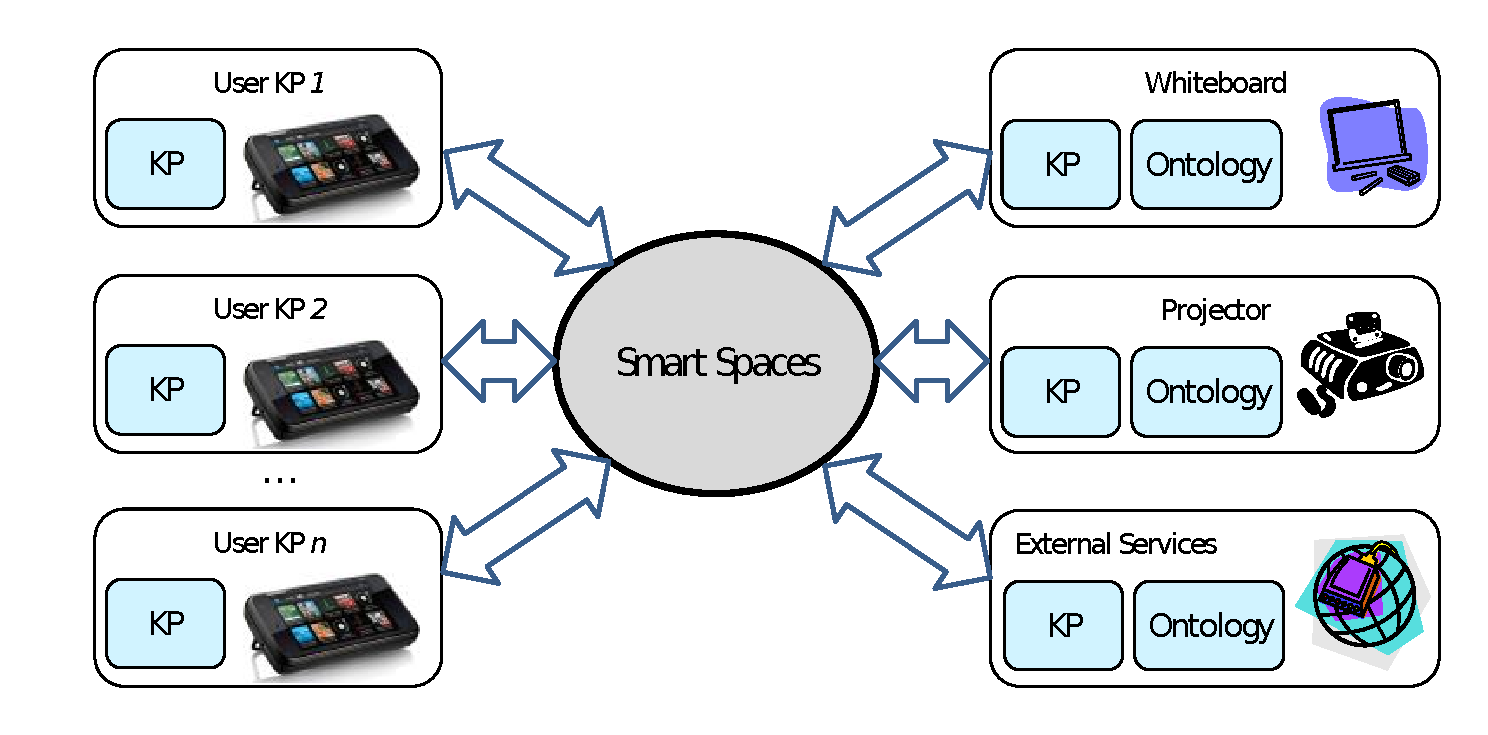
\epsfig{file=images/scs_arch.eps, width=17cm}}
\caption{Архитектура системы SC}
\label{scs-arch}
\end{figure}

Как и любое интеллектуальное приложение SC имеет распределённую архитектуру (рис.~\ref{scs-arch}). Система включает в себя три вида агентов.

{\bf 1. Проектор (projector)}.
Агент-проектор отображает текущий слайд презентации на экране конференции через мультимедиа проектор. Данные агент загружает файл с презентацией выступающего при начале выступления, а также осуществляет переход между слайдами презентации по требованию пользователя.

{\bf 2. Доска (whiteboard)}.
Агент-whiteboard отображает расписание конференции на общем экране (через мультимедиа проектор), уведомляет выступающего о том, что время выступления подходит к концу, отменяет презентацию пользователя, если данный участник отсутствует. Кроме этого агент позволяет председателю конференции изменять порядок участников.

{\bf 3. Клиент (SC-client)}.
Клиентский агент запускается на мобильном устройстве каждого участника конференции. Клиент отображает расписание конференции, позволяет просмотреть текущий слайд презентации, персональную информацию каждого участника, а также информацию о презентациях, позволяет изменять данные в пользовательском профиле. Выступающий участник имеет возможность управлять своей презентацией: осуществлять переход между слайдами.

%%%%%%%%%%%%%%%%
Каждый из агентов системы SC использует общее пространство конференции. Онтологическое описание пространства конференции представлено на рис. \ref{scs-ontology}. Оно состоит из трёх основных классов: менеджер пользовательской информации (user information manager), менеджер событий (event manager) и менеджер проектора (projector manager). Менеджер пользовательской информации хранит данные о профилях пользователей, видео выступающих, а также ссылку на текущий слайд. Кроме этого данный класс хранит информацию о расписании конференции и временных интервалах. Профиль пользователя содержит информацию о пользователе (имя, фото, электронный адрес, номер телефона, интересы, язык) и о презентации (имя презентации, ключевые слова и ссылка расположения презентации, для скачивания её другими агентами).
\begin{figure}[h]
\centerline{
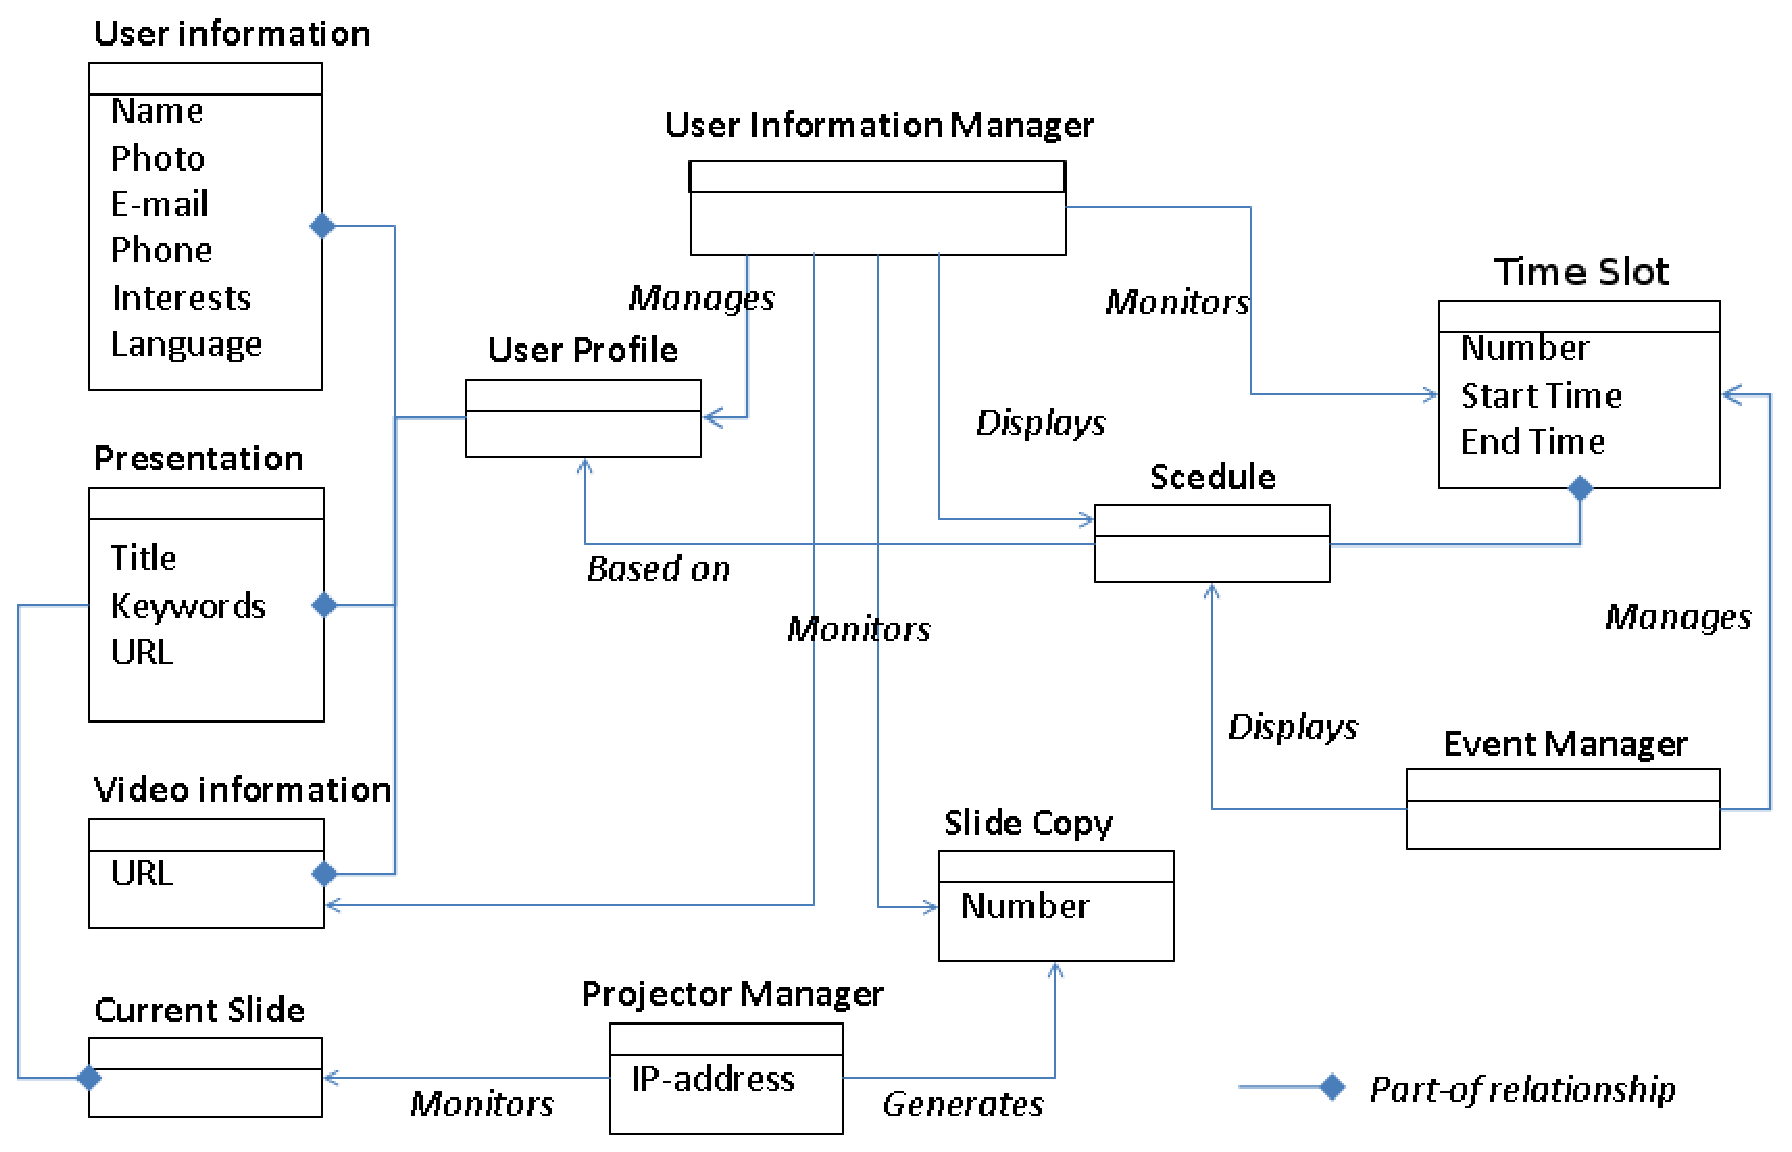
\epsfig{file=images/scs-ontology.eps, width=12cm}}
\caption{Онтология SCS}
\label{scs-ontology}
\end{figure}

Менеджер проектора создаёт скриншот и хранит ссылку на текущий слайд, который будет отображаться на экранах мобильных устройств. Менеджер событий содержит расписание конференции и управляет временными слотами. Расписание конференции создаётся в соответствии с профилями пользователей.
%%%%%%%%%%%%%%%%

Итак система SC является удобным интеллектуальным приложением для проведения конференций. Несмотря на это функционал данной системы может быть расширен при помощи других сервисов в ИП, что позволит проводить конференцию на более высоком уровне.

\subsection*{Идея интегрирования функций SmartScribo в систему SC}

Одним из таких дополнений может быть проведение дискуссий между участниками конференций. Помимо устных дискуссий после выступления расказчика, удобным также является проведение электронной онлайн дискуссии во время или после выступления. Часто при выступлении участника конференции у слушателя могут возникнуть вопросы, и в таком случае он может сразу опубликовать свой вопрос, а другие участники смогут его увидеть и, возможно, прокомментировать. Выступающий участник после выступления может зачитать и ответить на все вопросы. Кроме этого другие участники могут устроить дебаты на различные темы презентаций, в том числе и те, которые уже были рассказаны. Хорошим дополнением к этому является возможность клиента SC просмотреть полностью презентацию участника конференции и, таким образом, пользователь может вспомнить некоторые детали.

Нашей задачей являлась интеграция двух интеллектуальных приложений: SC и SmartScribo \cite{scblogging}. Внедрение возможностей блоггинга в конференцию позволило бы участникам вести нити дискуссий. Пост в блог конференции соответствует одному выступлению. Участники могут оставлять комментарии на пост (задавать вопросы) или отправлять комментарии на комментарии (отвечать на вопросы, дискутировать). Все участники могут просматривать и оставлять записи при помощи клиента SmartScribo со своих мобильных устройств. Блог-процессор SmartScribo будет синхронизировать данные дискуссии между ИП и блог-сервисом, поэтому пользователи также смогут принять участие в дискуссии, используя обычный веб-браузер. Таким образом ключевой задачей в интеграции двух приложений является координация между знаниями пространства конференции, блог-сервисом и пространством блогосферы.
%The key problem is coordination between the conference space, blog service, and blogosphere space.

Вследствие того, что не существует определённой схемы интеграции интеллектуальных приложений, для достижения этой цели можно применять два подхода:
\begin{enumerate}
\item Построение общей онтологии.
\item Использование агента-посредника.
\end{enumerate}

Первый подход основывается на построении общей онтологии, которая будет известна и будет использоваться всеми интегрируемыми интеллектуальными приложениями. В таком подходе оправдано использование стандартных онтологий, таких как FOAF для описания пользовательской информации. Таким образом онтология приложений будет представлять собой одно дерево зависимостей между классами знаний, а каждое приложение будет взаимодействовать с общим пространством, объединяющим онтологические данные из разных приложений.

Однако данный подход требует изначального знания общей онтологии разработчиками всех интегрируемых приложений, в противном случае готовое приложение необходимо будет модифицировать, что приведёт к дополнительным затратам.
Кроме этого использование общей онтологии не решает задачу синхронизации данных, когда между знаниями разных приложений существует некоторая функциональная зависимость. В таком случае преобразования данных должны выполнятся каким-либо агентом, что приводит к добавлению дополнительной функциональности, не требуемой при автономной работе одного из приложений.

Второй подход основывается на использовании некоторого агента-посредника, которые знает онтологии (или фрагменты онтологий) интегрируемых интеллектуальных приложений. В данном подходе каждое приложение имеет своё собственное независимое ИП. Агент-посредник ведёт наблюдение за знаниями нескольких приложений и в определённые моменты осуществляет требуемые операции. Такой агент выполняет синхронизацию данных между разными онтологиями (при добавлении или изменении в одной из них), а также осуществляет преобразование данных при различиях в представлениях одних и тех же данных в разных онтологиях или при наличии функциональной зависимости между знаниями.



При осуществлении интеграции функций блоггинга в конференцию был выбран второй подход: использование агента-посредника. Общая схема интеграции представлена на рис. \ref{scs-architecture}.
\begin{figure}[h]
\centerline{
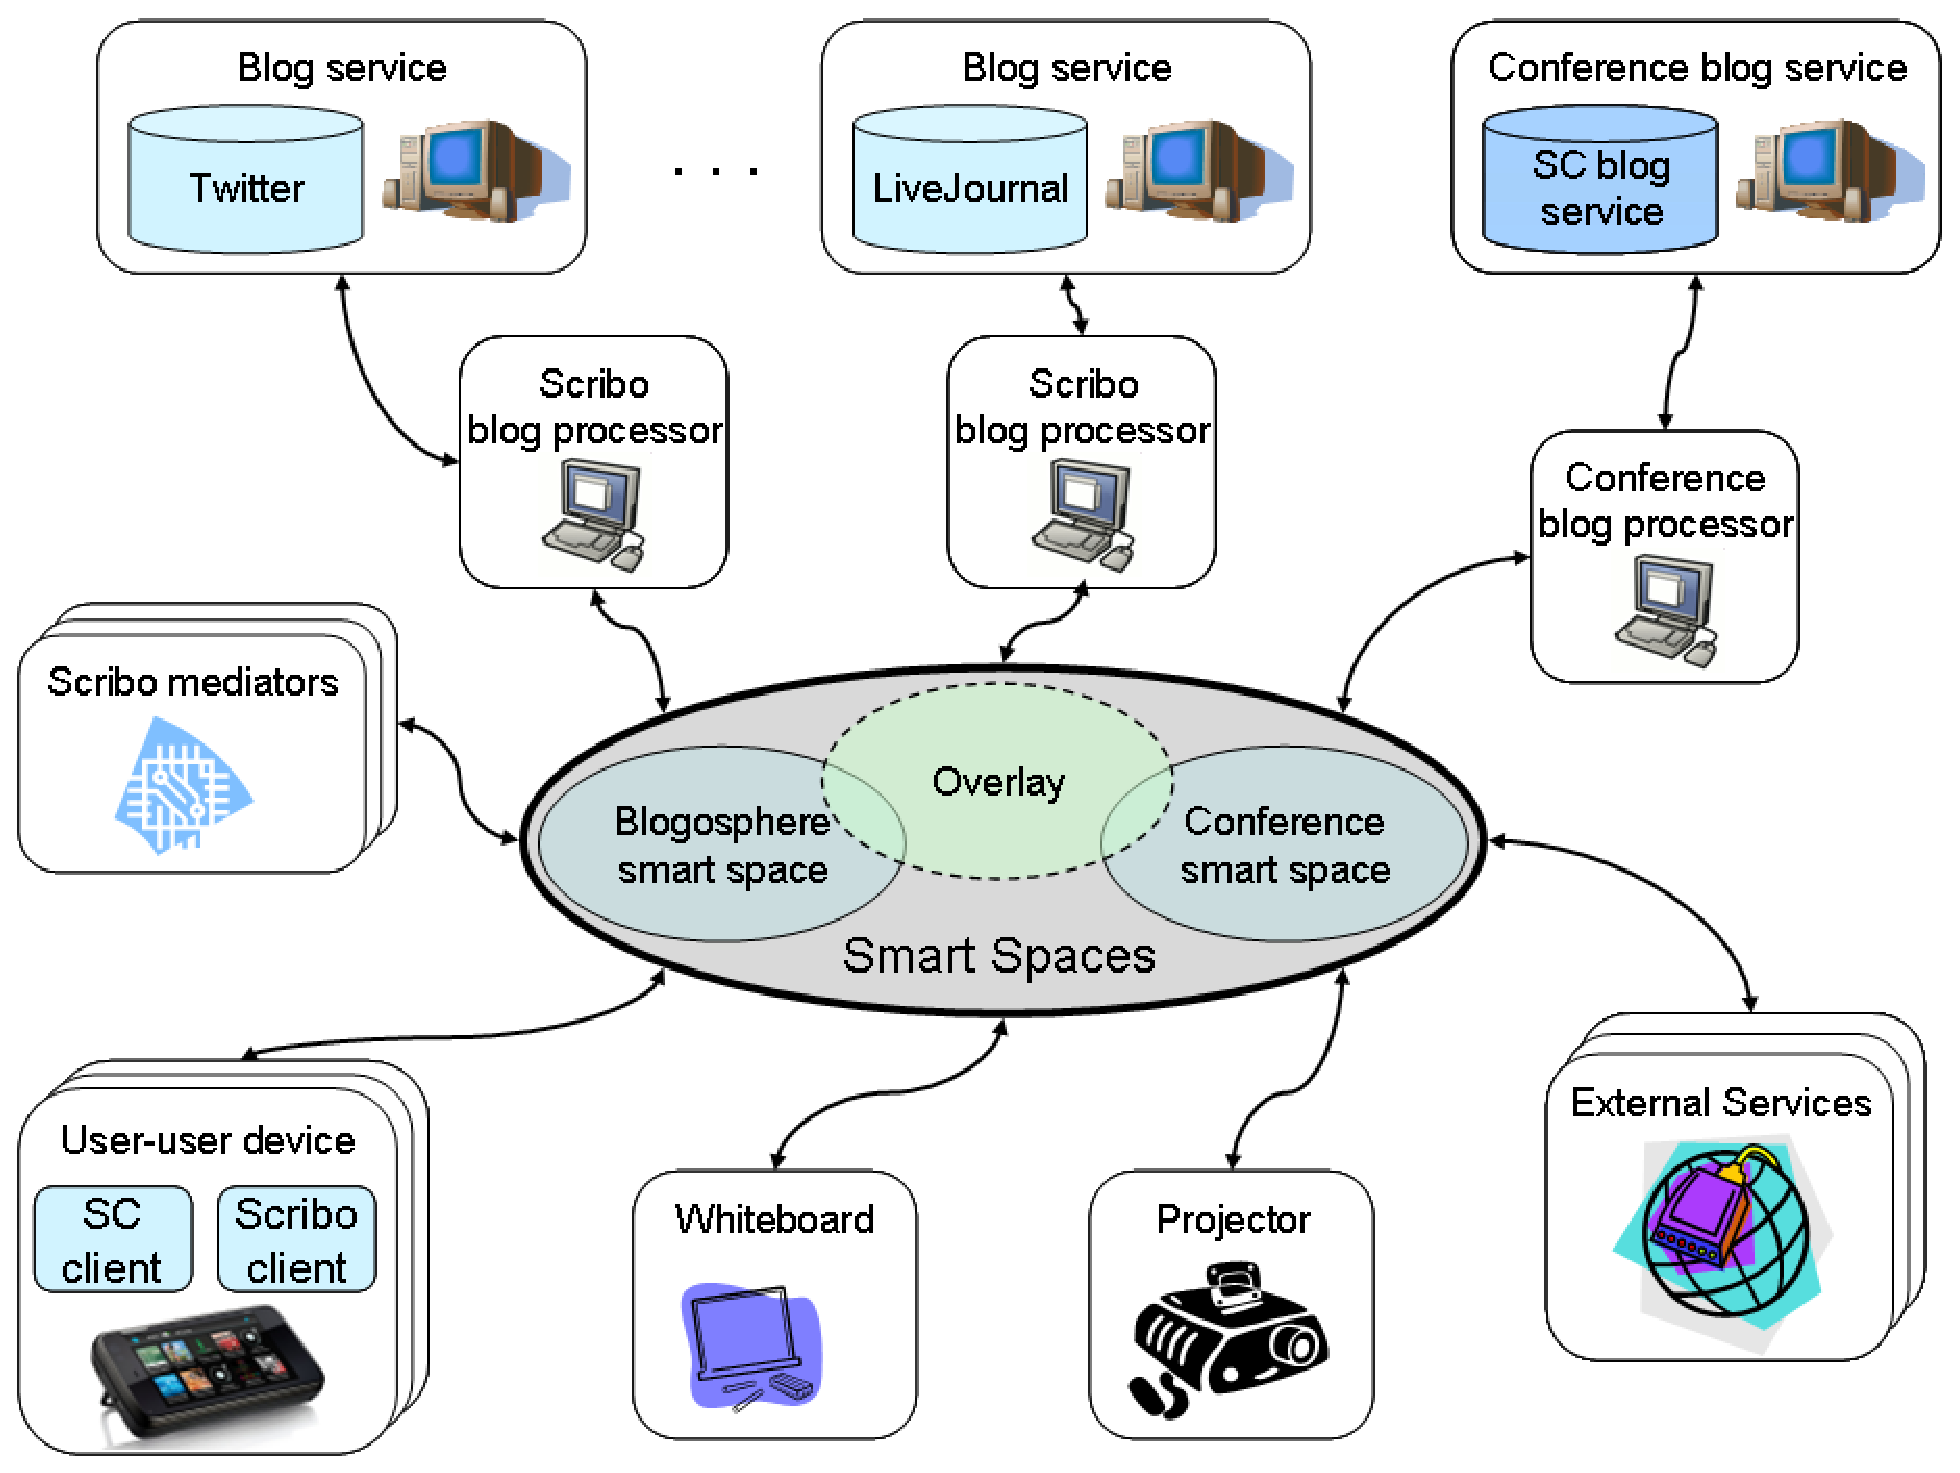
\epsfig{file=images/arch_scs.eps, width=14cm}}
\caption{Схема интеграции SCS и SmartScribo}
\label{scs-architecture}
\end{figure}

Для проведенния блог-дискуссий запускается собственный сервер, использующий блог-машину LiveJournal. Блог является первичным хранилищем всех дискуссий, связанных с конференцией.

Для каждой конференции система SC создаёт отдельный блог. Блог состоит из постов, каждый из которых соответствует одному выступлению. Также некоторые посты могут быть посвящены другим темам, связанным с конференцией, например обсуждение организации. Таким образом SC проходит стадию инициализации и определяет структуру дискуссий.

Для связи программы конференции и дискуссий используется блог-процессор SmartScribo в качестве агента-посредника. Данный агент следит за расписанием в пространстве конференции. При добавлении или изменении элементов расписания, агент отражает эти модификации на блог-сервисе. Связь между агентом-посредником и пространством конференции является однонаправленной, т.е. агент получает данные из SC и преобразует расписание в структуру блога.

Взаимодействие агента-посредника с пространством блогосферы реализуется так же, как и в обычных блог-процессорах SmartScribo. В отличие от связи агента с пространством конференции, связь с пространством блогов является двунаправленной, так как блог-процессор публикует в нём посты и комментарии, а также получает из него комментарии других пользователей и синхронизирует эти данные с блог-сервисом. В целях снижения влияния других пользователей на блог конференции все посты (а возможно и комментарии) публикуются от имени SC (абстрактного пользователя с правами администратора). Все остальные пользователи не имеют права модифицировать структуру блога конференции. В текущей реализации предполагается, что существует также один общий аккаунт для всех участников конференции, в дополнение к аккаунту администратора. Используя общий аккаунт пользователи могут оставлять комментарии анонимно, либо подписываться вконце сообщения. 

Для того, чтобы интегрирующий агент мог взаимодействовать с ИП различных приложений, он должен обладать знаниями о тех фрагментах онтологий, которые необходимы при выполнении сценариев интеграции. Следовательно, агент-посредник должен иметь некоторую оверлейную онтологию.

В общем случае оверлейная онтология --- это онтология, имеющая представление о фрагментах двух или более других онтологий. Такая онтология концептуально или онтологически связывает онтологии различных интеллектуальных приложений. Оверлейная онтология содержит данные других онтологий, которые могут быть одинаковы (в таком случае выполняется синхронизация этих данных), могут быть схожи (тогда определяется семантическая близость и могут выполнятся некоторые операции преобразования данных) или могут зависеть друг от друга (тогда выполняются соответствующие действия, разрешающие эту функциональную зависимость).

Для определения изменениий в покрываемых онтологиях могут использоваться два способа: подписка на сами данные, которые входят в оверлейную онтологию (и получение в дальнейшем их изменений) или запрос этих данных в начале работы, если в будущем данные не будут меняться); либо использование модели нотификаций, которая кроме инциирования действия у одного агента, позволяет сообщать также какие фрагменты онтологии (данных) были модифицированы. Однако об оповещении нотификацией должны заботиться те агенты, которые вносят изменения в данные. В случаях частого и массового изменения некоторых данных онтологии, выгоднее использовать нотификации, а не подписку на все эти данные.

Оверлейная онтология блог-процессора SC, содержащая фрагменты онтологии конференции и блогосферы, представлена на рис. \ref{bp-ontology}. Таким образом агент-посредник может отслеживать и синхронизировать знания между двумя интеллектуальными приложениями. При работе с онтологическими данными блогосферы блог-процессор использует нотификации. Однако текущая версия SC не поддерживает модель нотификаций, а также не позволяет коренным образом изменять расписание во время конференции (возможно только изменение порядка выступающих). В связи с этим агент-посредник не использует подписку на данные выступлений, т.к. они не изменяются, а получает их и преобразует в блог-структуру в начале работы.

\begin{figure}[h]
\centerline{
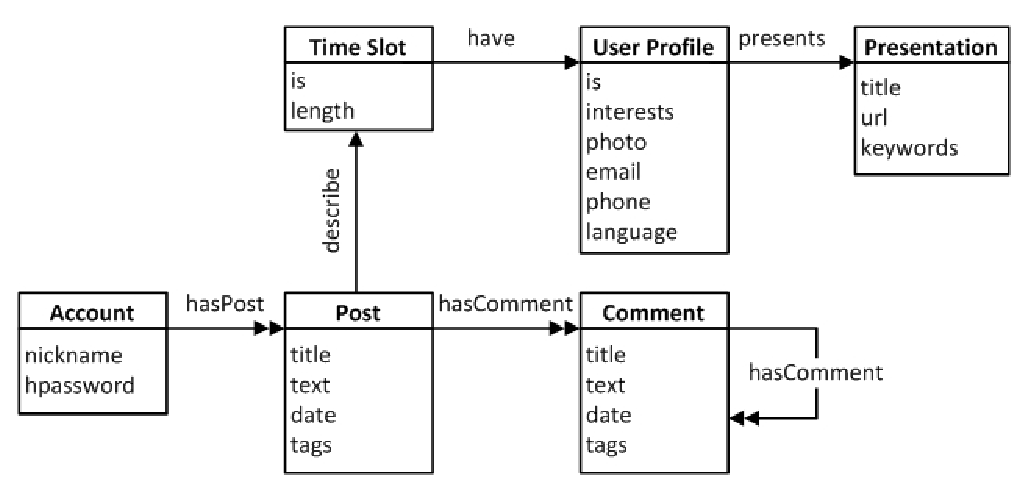
\epsfig{file=images/bp_ontology.eps, width=12cm}}
\caption{Оверлейная онтология блог-процессора}
\label{bp-ontology}
\end{figure}

В онтологиях конференции и блогосферы существует отношение один к одному между классами {\tt Post} из SmartScribo и {\tt TimeSlot} из SC. Свойство <<describe>> связывает эти классы. Данное свойство означает, что существует только один пост в блоге для каждого временного слота, соответствующего какому-либо выступлению. Такой пост содержит информацию о докладе, запланированном на указанное время.


\section{Интеграция с приложением M3-Weather}
\subsection*{Описание M3-Weather}
Приложение SmartScribo может взаимодействовать и с другими интеллектуальными приложениями. В данном разделе будет рассмотрена возможность использования в блоггинге контекстных данных пользователя и текущем местоположении и погоде.

Проект M3-Weather \cite{m3weather} представляет собой прототип туристического приложения.
Данное приложение при помощи глобальной системы позиционирования (Global
Positioning System, GPS) определяет координаты текущего месторасположения и,
используя их, отображает на экране пользовательского устройства прогноз погоды
для текущей местности. Процесс получения информации о погоде состоит из следующих действий.
\begin{enumerate}
\item
Определение текущих координат планшета с помощью GPS.
\item
Определение ближайшего населенного пункта.
\item
Определение и отображение прогноза погоды в текущей местности.
\item
Периодическое самостоятельное обновление данных о погоде.
\end{enumerate}

Согласно парадигме программирования ИП, приложение разбивается
на агенты, каждый из которых будет выполнять некоторую отдельную функцию.
Данные агенты в дальнейшем могут использоваться в других интеллектуальных
программах.

Архитектура M3-weather представлена на рис. \ref{m3w-arch}. Приложение может быть представлено в виде четырёх
агентов, два из которых работают на мобильном устройстве, а другие два — на
сервере. На устройстве запускается агент, взаимодействующий с GPS модулем, и агент, отображающий информацию о погоде на экране планшета. Следовательно на сервере должен работать агент, взаимодействующий с сервисом определения города по координатам, и агент, взаимодействующий с сервисом погоды. Перечислим функции, которые выполняет каждый из агентов.
\begin{figure}[h]
\centerline{
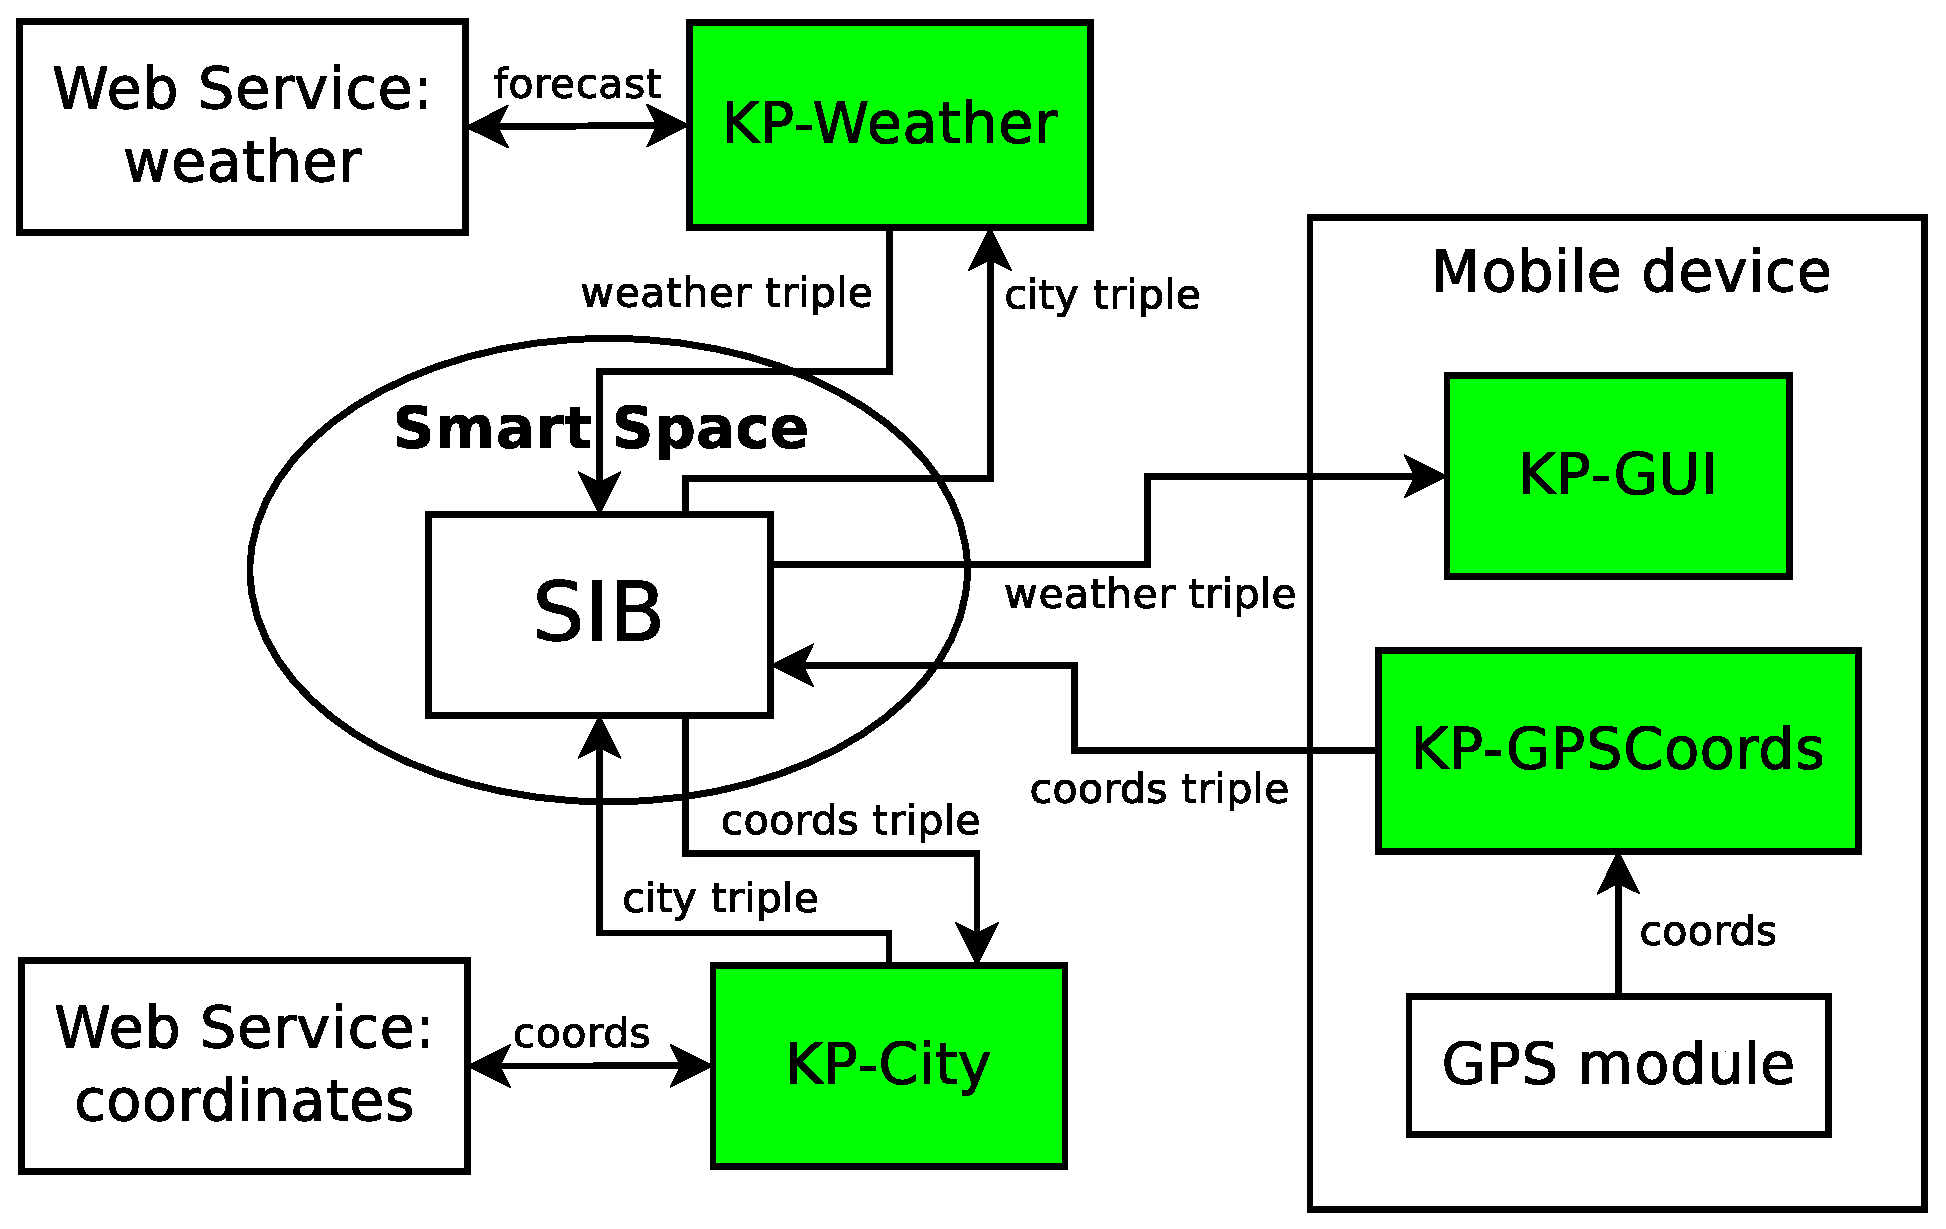
\epsfig{file=images/m3w_arch.eps, width=14cm}}
\caption{Архитектура M3-Weather}
\label{m3w-arch}
\end{figure}
\newpage
\begin{enumerate}
\item
Агент, взаимодействующий с GPS модулем (KP-GPSCoords)
\begin{itemize}
\item
получение с помощью GPS модуля координаты текущего месторасположения
\item
периодическое обновление координат
\item
сохранение полученных координат в SIB
\end{itemize}
\item
Агент, взаимодействующий с веб-сервисом определения города по координатам (KP-City)
\begin{itemize}
\item
получение текущих координат месторасположения из SIB
\item
отправка полученных координат веб-сервису и получение названия ближайшего города
\item
сохранение полученных данных о городе в SIB
\end{itemize}
\item
Агент, взаимодействующий с веб-сервисом прогноза погоды (KP-Weather)
\begin{itemize}
\item
получение текущего названия города из SIB
\item
отправка названия города веб-сервису и получение информации о погоде в этом городе
\item       
сохранение информации о погоде в SIB
\end{itemize}
\item
Агент, взаимодействующий с экраном планшета (KP-GUI)
\begin{itemize}
\item
получение актуальных данных о городе и погоде из SIB
\item
отображение на экране планшета информации о городе и погоде
\end{itemize}
\end{enumerate}

Для того, чтобы агенты могли взаимодействовать между
собой, необходим общий формат данных, который бы полностью описывал предметную область
и позволял представлять информацию в ИП.

Онтология M3-Weather (рис. \ref{m3w-ontology}) представляет собой структурированное описание данных о координатах, городе и погоде. В онтологии выделяется три основных класса: координаты ({\tt Coords}), город ({\tt City}) и погода ({\tt Weather}). Стрелка с надписью {\tt type} указывает на тип сущности (в данном случае объекты являются классами). Каждый класс обладает свойствами,
которые имеют тип {\tt DatatypeProperty}. Стрелка с надписью {\tt domain} обозначает, к какому объекту относится указанное свойство. Рассмотрим подробнее назначение каждого свойства.
\begin{figure}[h]
\centerline{
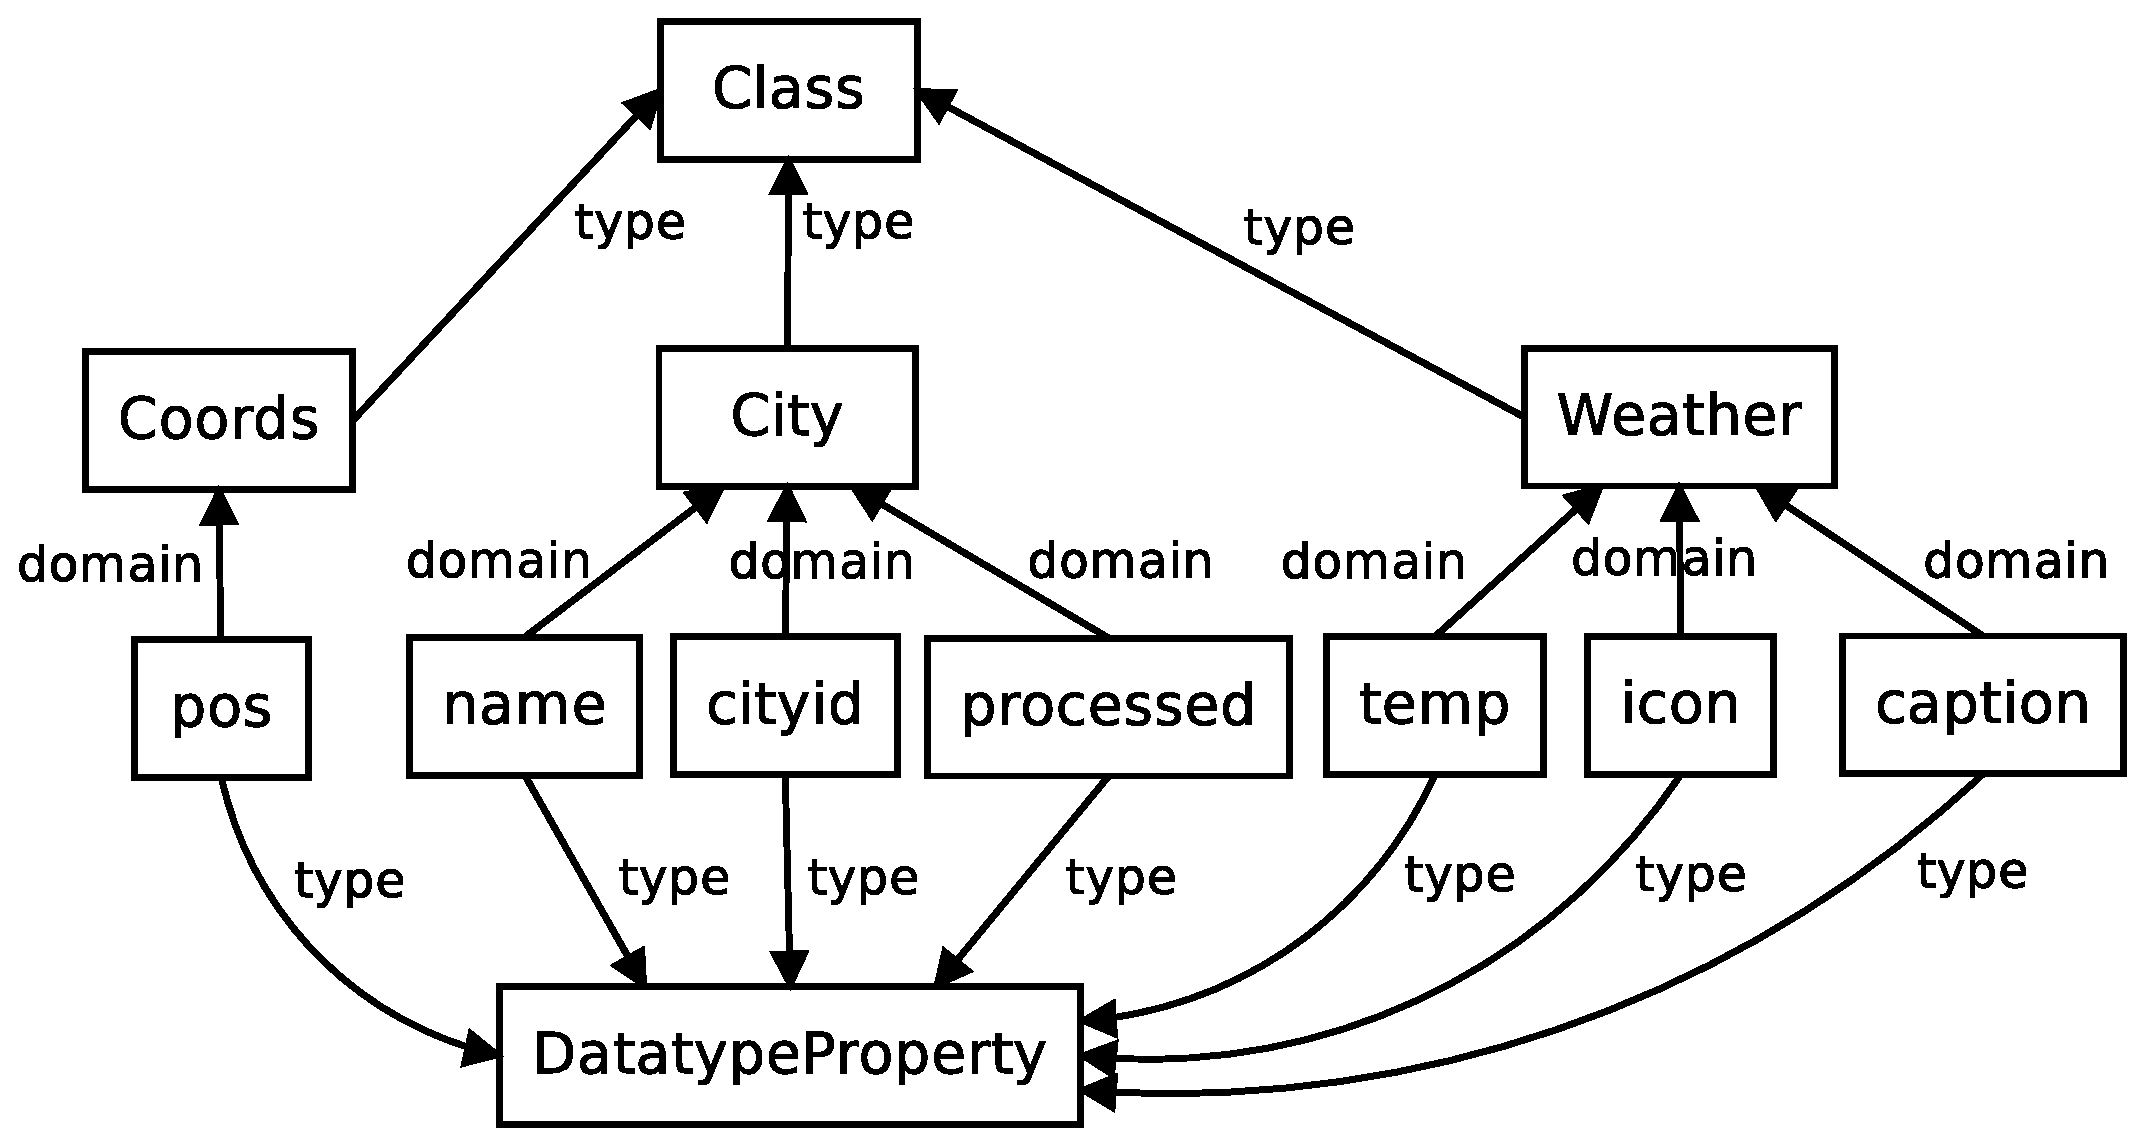
\epsfig{file=images/m3w-ontology.eps, width=14cm}}
\caption{Онтология M3-Weather}
\label{m3w-ontology}
\end{figure}

\vspace{-0.9cm}
\begin{enumerate}
\item
класс {\tt Coords}\\
обладает только одним свойством {\tt pos}, которое хранит данные о текущем местоположении (широта и долгота)
\item
класс {\tt City}
\begin{itemize}
\item
свойство {\tt name} хранит название ближайшего города
\item
свойство {\tt cityid} предназначено для хранения идентификатора города, используемого
для определения погоды на веб-сервисе
\item
свойство {\tt processed} содержит информацию о том, был ли найден прогноз погоды для данного города (значение yes или no)
\end{itemize}
\item
класс {\tt Weather}
\begin{itemize}
\item
свойство {\tt temp} содержит температуру
\item
свойство {\tt icon} содержит номер иконки, иллюстрирующей погоду
\item
свойство {\tt caption} содержит краткое описание погоды
\end{itemize}
\end{enumerate}

Для хранения конкретных данных в онтологии, необходимо создать индивида класса.
Описание индивида представляет собой триплет вида ``<имя\_индивида>, type, <класс>".
Для установки значения свойства индивида задаётся триплет вида
``<имя\_индивида>, <имя\_свойства>, <значение>".

Онтология M3-Weather позволяет хранить многопользовательские данные. Чтобы представить данные нескольких пользователей, каждому пользовательскому устройству присваивается уникальный идентификатор. При создании индивидов каждого из классов онтологии к имени индивида добавляется данный идентификатор. Таким образом устройство сможет получить данные, предназначенные только для него.

Рассмотрим порядок взаимодействия между всеми агентами, а также взаимодействие с онтологическими данными. Напомним, что обмен данными между агентами осуществляется при помощи механизма публикации и подписки.

KP-GPSCoords получает данные о текущем месторасположении от GPS-модуля и записывает их в индивид класса {\tt Coords} в SIB с некоторой периодичностью. 
При публикации данных генерируется триплет вида {\tt coords<id>~-~pos~-~<lat>;<lon>},
где {\tt <id>} --- это уникальный идентификатор пользовательского устройства,
{\tt <lat>} --- широта, а {\tt <lon>} --- долгота.

KP-City подписывается на индивидов класса {\tt Coords} (триплеты, публикуемые KP-GPSCoords). 
При появлении в SIB новых координат или при изменении существующих,
агент получает эти данные и отправляет запрос с координатами веб-сервису геокодирования.
Сервер возвращает список ближайших к данному местоположению городов. Из списка выбирается наиболее ближайший город и далее отправляется запрос с названием города веб-сервису погоды.
Если город присутствует в базе данных веб-сервиса погоды, то возвращается его идентификатор.
При отсутствии города в базе данных выбирается следующий ближайший город из списка, и процесс
повторяется, пока не будет получен идентификатор.

После получения необходимых данных, KP-City публикует их в SIB, как свойства индивида {\tt City}. Также к индивиду добавляется свойство {\tt processed} со значением {\tt no}. Это
свойство показывает, что для данного индивида ещё не был определён прогноз погоды. 

KP-Weather подписан на индивидов класса {\tt City}, имеющих значение свойства
{\tt processed -- no}. При появлении такого индивида, агент получает идентификатор города
и отправляет запрос на веб-сервис погоды для получения прогноза. При получении данных о погоде, он публикует их в SIB, а также меняет у индивида {\tt City} значение свойства {\tt processed} на {\tt yes}.

KP-GUI работает на устройстве и имеет графический интерфейс. Агент подписан на индивидов
классов {\tt City} и {\tt Weather} и, при их создании или обновлении, отображает на экране устройства актуальные данные о текущем городе и погоде.

\subsection*{Использование данных M3-Weather в SmartScribo}

Данные, получаемые приложением M3-Weather, можно использовать в других интеллектуальных приложениях. Например данные о текущих координатах, городе или погоде могут быть использованы в блог-клиенте SmartScribo при отправке поста в собственный блог во время путешествия.

Интеграцию данных M3-Weather в SmartScribo можно осуществить при помощи создания общей онтологии. Вследствие того, что информация о координатах, текущем городе и погоде является контекстом пользователя, а в онтологии SmartScribo в профиле пользователя существует класс {\tt Context}, то достаточно добавить в этом классе свойства, связывающие контекстную информацию блоггера с данными M3-Weather.

Данные, публикуемые M3-Weather, представляют собой набор триплетов, субъекты которых соответствуют трём классам знаний: координаты (coords<id>), город (city<id>), погода (weather<id>). Все три индивида содержат в своём названии одинаковый идентификатор {\tt id}, который является уникальным идентификатором пользовательского устройства в ИП. Таким же идентификатором может обладать профиль пользователя в онтологии SmartScribo. Таким образом агенты M3-Weather могут записывать свои данные в персональное пространство блоггера.

Объединение онтологий указанных интеллектуальных приложений достигается путём добавления связей между контекстом (индивидом контекста у профиля пользователя) и индивидами M3-Weather. Пусть свойство <<curCoords>> связывает контекст с координатами, <<curCity>> -- с текущим городом и <<curWeather>> с текущей погодой. Триплеты которые публикуют агенты M3-Weather имеют вид:
$$
\begin{array}{l}
\mbox{coords-<id>}, \mbox{pos}, \mbox{<coordinates>}\\
\mbox{city-<id>}, \mbox{name}, \mbox{<cityname>}\\
\mbox{weather-<id>}, \mbox{temp}, \mbox{<temperature>}\\
...
\end{array}
$$
где <coordinates>, <cityname>, <temperature> --- конкретные значения соответствующих свойств. Для связки контекстных данных блоггера с данными M3-Weather, агенты обращаются к профилю блоггера {\tt profile-<id>}, через свойство <<hasContext>> получают доступ к индивиду контекста и публикуют следующие триплеты:
$$
\begin{array}{l}
\mbox{context-<id>}, \mbox{curCoords}, \mbox{coords-<id>}\\
\mbox{context-<id>}, \mbox{curCity}, \mbox{city-<id>}\\
\mbox{context-<id>}, \mbox{curWeather}, \mbox{weather-<id>}
\end{array}
$$
Таким образом данные о координатах, городе и погоде становятся контекстом блоггера. Агенты SmartScribo могут получать эти данные через индивида класса {\tt Context}. Такая информация может быть автоматически вставлена в сообщение при написании поста во время путешествия.
